\documentclass[12pt]{article}
\usepackage[margin=0.1in]{geometry}
\usepackage{arev}
\usepackage{pgfplots}
\usetikzlibrary{calc}
\pgfplotsset{compat=newest}

\definecolor{colour1}{RGB}{240, 167, 116}
\definecolor{colour2}{RGB}{232, 93, 73}
\definecolor{colour3}{RGB}{135, 0, 97}

\begin{document}

% First example of the notes
\begin{figure}[hbt]
    \centering
    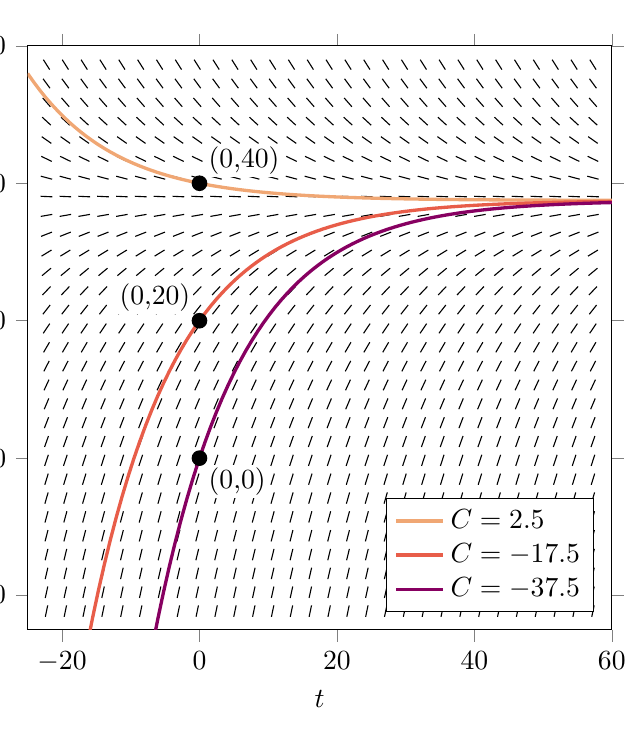
\begin{tikzpicture}[
        trim axis left, trim axis right, % options to centre correctly
        declare function={
            dydx(\x,\y) = 3-0.08*\y; % differential equation
            solution(\x,\c) = 37.5+\c*exp(-0.08*\x); % general solution
        }]

        % domain and tick settings - note domain is square, change in axis options if needed
        \def\domainMin{-25} \def\domainMax{60}
        \def\ticks{\domainMin+5,\domainMin+25,...,\domainMax} % define tick marks
        \def\width{9cm} \def\height{9cm}
        \pgfmathsetmacro{\scale}{(\domainMax-\domainMin)/50} % scale of the slopes

        % #1: coordinates of node, #2: relative position of node label (can also be angle)
        \newcommand\labelledPoint[2]{\node[circle, fill, inner sep=2pt, label={[fill=white,distance=1pt,inner sep=1pt]#2:{(#1)}}] at (#1){}}

        % Dummy axis plot: https://tex.stackexchange.com/questions/170664/
        \begin{axis}[xmin=\domainMin, xmax=\domainMax, ymin=\domainMin, ymax=\domainMax, width=\width, height=\height, hide axis]
            \coordinate (O) at (axis cs:0,0); \coordinate (X) at (axis cs:1,0); \coordinate (Y) at (axis cs:0,1);
        \end{axis}

        % Extraction of axis coordinates and plotting slope fields
        \begin{scope}[x={($(X)-(O)$)}, y={($(Y)-(O)$)}, shift={(O)}]
        \def\numSlopes{30}
        \pgfmathsetmacro{\h}{(\domainMax-\domainMin)/(\numSlopes+1)}
        \pgfmathsetmacro{\totalSlopes}{\numSlopes^2-1}
        \foreach \i [evaluate=\i as \x using \domainMin+\i*\h] in {1,...,\numSlopes} {
            \foreach \j [evaluate=\j as \y using \domainMin+\j*\h] in {1,...,\numSlopes} {
                \pgfmathsetmacro{\slope}{dydx(\x,\y)};
                \pgfmathsetmacro{\dx}{\scale/sqrt((\slope)^2+1)};
                \pgfmathsetmacro{\dy}{\slope*\dx};
                \draw[thin] ({\x-\dx/2}, {\y-\dy/2})--({\x+\dx/2}, {\y+\dy/2});
            };
        };
        \end{scope}

        % Axis where solutions are plotted
        \begin{axis}[view = {0}{90}, % set camera to point towards x-y plane
                     domain=\domainMin:\domainMax,
                     xmin=\domainMin, xmax=\domainMax,
                     ymin=\domainMin, ymax=\domainMax,
                     xlabel=$t$, ylabel=$w$,
                     xtick=\ticks, ytick=\ticks,
                     tick align=outside,
                     width=\width, height=\height,
                     legend pos=south east, legend cell align={left},
                     axis equal image]

            % plot initial points and corresponding solution curves
            \addplot[very thick, colour1, samples=100] {solution(x, 2.5)};
            \labelledPoint{0,40}{above right};

            \addplot[very thick, colour2, samples=100] {solution(x, -17.5)};
            \labelledPoint{0,20}{above left};

            \addplot[very thick, colour3, samples=100] {solution(x, -37.5)};
            \labelledPoint{0,0}{below right};

            % add legend, ignoring quiver plot
            \legend{$C=2.5$, $C=-17.5$, $C=-37.5$}
        \end{axis}
    \end{tikzpicture}
    \caption{Slope field of $\frac{\mathrm{d}w}{\mathrm{d}t}=3-0.08w$, with solutions $w(t)=Ce^{-0.08t}+37.5$}
\end{figure}

% Second example of the notes
\begin{figure}[hbt]
    \centering
    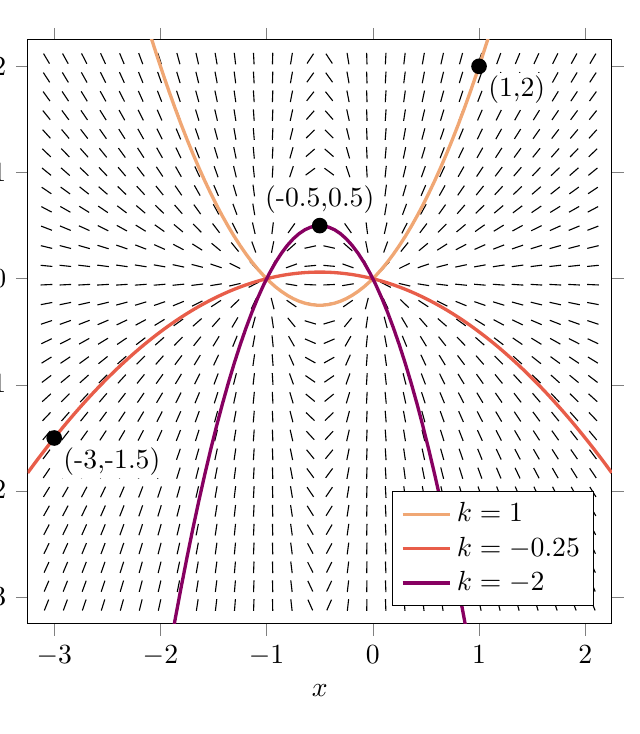
\begin{tikzpicture}[
        trim axis left, trim axis right, % options to centre correctly
        declare function={
            dydx(\x,\y) = (2*\x+1)*\y / ((\x)^2+\x); % differential equation
            solution(\x,\c) = \c*((\x)^2+\x); % general solution
        }]

        % domain and tick settings - note domain is square, change in axis options if needed
        \def\domainMin{-3.25} \def\domainMax{2.25}
        \def\ticks{\domainMin+0.25,...,\domainMax-0.25} % define tick marks
        \def\width{9cm} \def\height{9cm}
        \pgfmathsetmacro{\scale}{(\domainMax-\domainMin)/50} % scale of the slopes

        % #1: coordinates of node, #2: relative position of node label (can also be angle)
        \newcommand\labelledPoint[2]{\node[circle, fill, inner sep=2pt, label={[fill=white,distance=1pt,inner sep=1pt]#2:{(#1)}}] at (#1){}}

        % Dummy axis plot: https://tex.stackexchange.com/questions/170664/
        \begin{axis}[xmin=\domainMin, xmax=\domainMax, ymin=\domainMin, ymax=\domainMax, width=\width, height=\height, hide axis]
            \coordinate (O) at (axis cs:0,0); \coordinate (X) at (axis cs:1,0); \coordinate (Y) at (axis cs:0,1);
        \end{axis}

        % Extraction of axis coordinates and plotting slope fields
        \begin{scope}[x={($(X)-(O)$)}, y={($(Y)-(O)$)}, shift={(O)}]
        \def\numSlopes{30}
        \pgfmathsetmacro{\h}{(\domainMax-\domainMin)/(\numSlopes+1)}
        \pgfmathsetmacro{\totalSlopes}{\numSlopes^2-1}
        \foreach \i [evaluate=\i as \x using \domainMin+\i*\h] in {1,...,\numSlopes} {
            \foreach \j [evaluate=\j as \y using \domainMin+\j*\h] in {1,...,\numSlopes} {
                \pgfmathsetmacro{\slope}{dydx(\x,\y)};
                \pgfmathsetmacro{\dx}{\scale/sqrt((\slope)^2+1)};
                \pgfmathsetmacro{\dy}{\slope*\dx};
                \draw[thin] ({\x-\dx/2}, {\y-\dy/2})--({\x+\dx/2}, {\y+\dy/2});
            };
        };
        \end{scope}

        \begin{axis}[view = {0}{90}, % set camera to point towards x-y plane
                     domain=\domainMin:\domainMax,
                     xmin=\domainMin, xmax=\domainMax,
                     ymin=\domainMin, ymax=\domainMax,
                     xlabel=$x$, ylabel=$y$,
                     xtick=\ticks, ytick=\ticks,
                     tick align=outside,
                     width=\width, height=\height,
                     legend pos=south east, legend cell align={left},
                     axis equal image]

            % plot initial points and corresponding solution curves
            \addplot[very thick, colour1, samples=100] {solution(x, 1)};
            \labelledPoint{1,2}{below right};

            \addplot[very thick, colour2, samples=100] {solution(x, -0.25)};
            \labelledPoint{-3,-1.5}{below right};

            \addplot[very thick, colour3, samples=100] {solution(x, -2)};
            \labelledPoint{-0.5,0.5}{above};

            % % add legend, ignoring quiver plot
            \legend{$k=1$, $k=-0.25$, $k=-2$}
        \end{axis}
    \end{tikzpicture}
    \caption{Slope field of $\frac{\mathrm{d}y}{\mathrm{d}x}=k(2x+1)$, with solutions $y(x)=k(x^2+x)$}
\end{figure}

% % Example 13-5 on page 14
\begin{figure}[hbt]
    \centering
    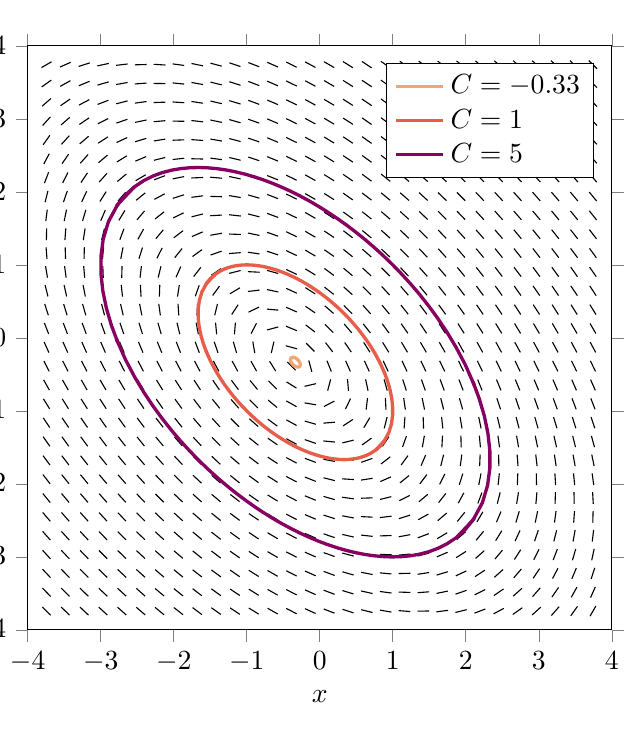
\begin{tikzpicture}[
        trim axis left, trim axis right, % options to centre correctly
        declare function={
            dydx(\x,\y) = -(2*\x+\y+1) / (\x+2*\y+1); % differential equation
        }]

        % domain and tick settings - note domain is square, change in axis options if needed
        \def\domainMin{-4} \def\domainMax{4}
        \def\ticks{\domainMin,...,\domainMax} % define tick marks
        \def\width{9cm} \def\height{9cm}
        \pgfmathsetmacro{\scale}{(\domainMax-\domainMin)/50} % scale of the slopes

        % #1: coordinates of node, #2: relative position of node label (can also be angle)
        \newcommand\labelledPoint[2]{\node[circle, fill, inner sep=2pt, label={[fill=white,distance=1pt,inner sep=1pt]#2:{(#1)}}] at (#1){}}

        % #1: integration constant c, #2: colour
        % The solution relation is x^2 + y^2 + xy + x + y = C. Rearrange for
        % y = ±f(x) and x = ±f(y), note the symmetry. Plot all 4 equations with
        % some padding to reduce overlap and regions of low resolution. All this
        % is to plot a continuous curve without using an insane amount of samples.
        % I couldn't manage to parametrise the relation.
        \newcommand\ellipse[2]{
            \pgfmathsetmacro{\lowerBound}{-1/3 * (1+2*sqrt(3*(#1)+1))}
            \pgfmathsetmacro{\upperBound}{-1/3 * (1-2*sqrt(3*(#1)+1))}
            \pgfmathsetmacro{\padding}{0.2 * (\upperBound-\lowerBound)}
            \pgfmathsetmacro{\lowerApex}{-(\lowerBound+1)/2} % apex of the ellipse (intersection with y=-(x+1)/2
            \pgfmathsetmacro{\upperApex}{-(\upperBound+1)/2}
            \addplot[very thick, #2, samples=40, domain={\lowerBound+0.2*\padding}:{\upperBound-0.2*\padding}] plot (\x,{-0.5*(\x+1)+sqrt((#1)-0.25*(\x+1)*(3*\x-1))});
            \addplot[very thick, #2, samples=40, domain={\lowerBound+0.2*\padding}:{\upperBound-0.2*\padding},forget plot] plot (\x,{-0.5*(\x+1)-sqrt((#1)-0.25*(\x+1)*(3*\x-1))});
            \addplot[very thick, #2, samples=10, domain={\lowerApex-\padding}:{\lowerApex+\padding}, variable=\y,forget plot]  plot ({-0.5*(\y+1)-sqrt((#1)-0.25*(\y+1)*(3*\y-1))}, {\y});
            \addplot[very thick, #2, samples=10, domain={\upperApex-\padding}:{\upperApex+\padding}, variable=\y,forget plot]  plot ({-0.5*(\y+1)+sqrt((#1)-0.25*(\y+1)*(3*\y-1))}, {\y});
        }

        % Dummy axis plot: https://tex.stackexchange.com/questions/170664/
        \begin{axis}[xmin=\domainMin, xmax=\domainMax, ymin=\domainMin, ymax=\domainMax, width=\width, height=\height, hide axis]
            \coordinate (O) at (axis cs:0,0); \coordinate (X) at (axis cs:1,0); \coordinate (Y) at (axis cs:0,1);
        \end{axis}

        % Extraction of axis coordinates and plotting slope fields
        \begin{scope}[x={($(X)-(O)$)}, y={($(Y)-(O)$)}, shift={(O)}]
        \def\numSlopes{30}
        \pgfmathsetmacro{\h}{(\domainMax-\domainMin)/(\numSlopes+1)}
        \pgfmathsetmacro{\totalSlopes}{\numSlopes^2-1}
        \foreach \i [evaluate=\i as \x using \domainMin+\i*\h] in {1,...,\numSlopes} {
            \foreach \j [evaluate=\j as \y using \domainMin+\j*\h] in {1,...,\numSlopes} {
                \pgfmathsetmacro{\slope}{dydx(\x,\y)};
                \pgfmathsetmacro{\dx}{\scale/sqrt((\slope)^2+1)};
                \pgfmathsetmacro{\dy}{\slope*\dx};
                \draw[thin] ({\x-\dx/2}, {\y-\dy/2})--({\x+\dx/2}, {\y+\dy/2});
            };
        };
        \end{scope}

        \begin{axis}[view = {0}{90}, % set camera to point towards x-y plane
                     domain=\domainMin:\domainMax,
                     xmin=\domainMin, xmax=\domainMax,
                     ymin=\domainMin, ymax=\domainMax,
                     xlabel=$x$, ylabel=$y$,
                     xtick=\ticks, ytick=\ticks,
                     tick align=outside,
                     width=9cm, height=9cm,
                     legend pos=north east, legend cell align={left},
                     axis equal image]

            % solutions
            \ellipse{-0.33}{colour1}
            \ellipse{1}{colour2}
            \ellipse{5}{colour3}

            % add legend, ignoring quiver plot
            \legend{$C=-0.33$, $C=1$, $C=5$}
        \end{axis}
    \end{tikzpicture}
    \caption{Slope field of $\frac{\mathrm{d}y}{\mathrm{d}x}=-\frac{2x+y+1}{x+2y+1}$, with solutions $x^2+y^2+xy+x+y=C\geq-\frac13$}
\end{figure}
\end{document}
